%Synthèse des résultats. On utilisera des graphiques (histogrammes, camemberts, etc.) pour faciliter la lecture.
%Les résultats seront fournis sous forme de fichiers texte au format CSV ou . 

La simulation a été exécutée sur 4 scénarios. Chaque scénario durait 90 jours, et voyait des avions arriver avec des probabilités identiques :
\begin{itemize}
  \item Un avion toutes les 20 minutes en moyenne en horaire normal.
  \item Un avion toutes les 10 minutes en heure de pointe : de 7h à 10h et de 17h à 19h, en semaine.
  \item Un avion toutes les 40 minutes le week-end.
  \item Aucun avion de 22h à 7h.
\end{itemize}
Toutes les avions ont le même comportement, tel que décrit dans la modélisation du problème.

Les quatre scénarios ont pour seule différences le nombre de portes d'embarquement instanciées : 4, 6, 8 ou 12.

On étudie les horaires de notification des avions à la tour de contrôle et de début de phase d'approche. La différence entre ces deux dates indique le retard de l'avion, c'est à dire le temps que l'avion a passé en l'air à attendre la permission d'atterrir. Les moyennes de ces retards sont compilés dans le tableau \ref{retard_moyen}

\begin{table}[h]
\begin{center}
\begin{tabular}{|l|c|c|r|}
  \hline
  4 portes & 6 portes & 8 portes & 12 portes \\
  \hline
  123:12:35 & 544:06:03 & 356:29:14 & 0:08:10\\
  \hline
\end{tabular}
   \caption{\label{retard_moyen} Retard moyen}
\end{center}
\end{table}

\section{Retard en fonction du nombre de portes}
Voici ci dessous des répartitions plus détaillées des retards en fonction du nombre de portes:

\subsection{Aéroport à 4 portes d'embarquement}
La répartition des retards pour un aéroport à 4 portes,en pourcentage d'avions dans des intervalles de retards est donnée en figure~\ref{retard_camenbert_4}.
  \graphicspath{{donnees/graph_90jours/4portes/}}
\begin{figure}[H]
 \centering 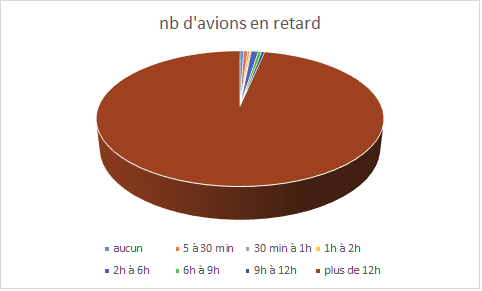
\includegraphics[scale=0.6]{retard_avions.png}
 \caption{\label{retard_camenbert_4} Répartition des retards, avec 4 portes} 
\end{figure}
 
 Une autre donnée intéressante est la répartition des retards par jour, donnée par la figure~\ref{retard_jour_4}
\begin{figure}[H]
\centering 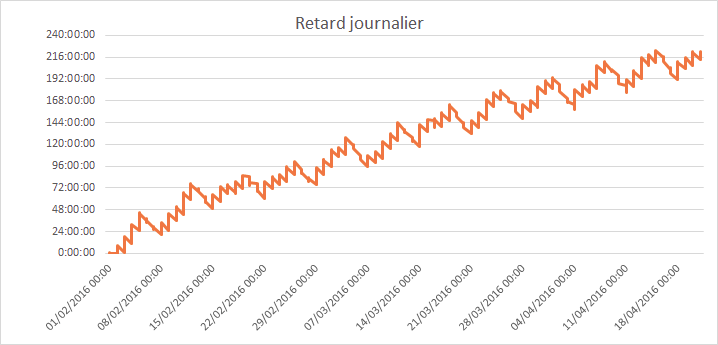
\includegraphics[scale=0.6]{retard_jours.png}
 \caption{\label{retard_jour_4} Retard avec 4 portes} 
\end{figure}
 
 \subsection{Aéroport à 6 portes d'embarquement}
La répartition des retards pour un aéroport à 6 portes,en pourcentage d'avions dans des intervalles de retards est donnée en figure~\ref{retard_camenbert_6}.
  \graphicspath{{donnees/graph_90jours/6portes/}}
\begin{figure}[H]
\centering 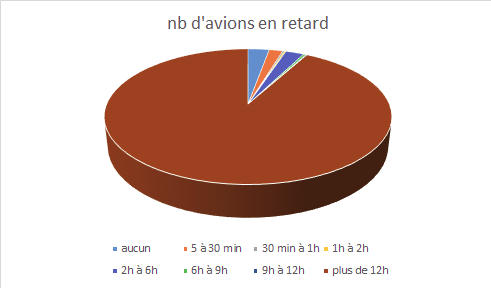
\includegraphics[scale=0.6]{retard_avions.png}
 \caption{\label{retard_camenbert_6} Répartition des retards, avec 6 portes} 
\end{figure}
 
 Une autre donnée intéressante est la répartition des retards par jour, donnée par la figure~\ref{retard_jour_6}
\begin{figure}[H]
\centering 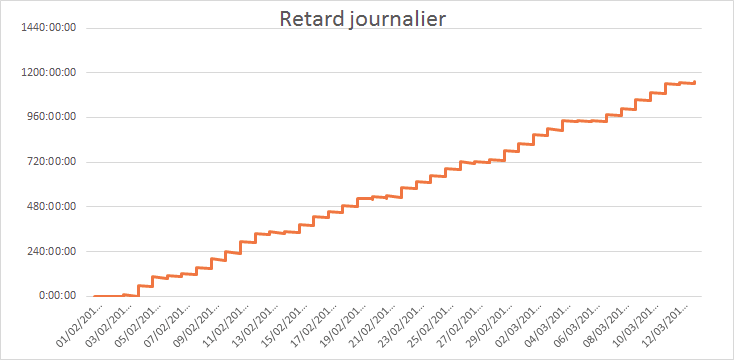
\includegraphics[scale=0.6]{retard_jour.png}
 \caption{\label{retard_jour_6} Retard avec 6 portes} 
\end{figure}
 
 \subsection{Aéroport à 8 portes d'embarquement}
La répartition des retards pour un aéroport à 8 portes,en pourcentage d'avions dans des intervalles de retards est donnée en figure~\ref{retard_camenbert_8}.
  \graphicspath{{donnees/graph_90jours/8portes/}}
\begin{figure}[H]
\centering 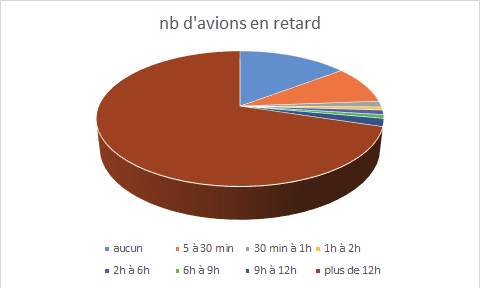
\includegraphics[scale=0.6]{retard_avions.png}
 \caption{\label{retard_camenbert_8} Répartition des retards, avec 8 portes} 
\end{figure}
 
 Une autre donnée intéressante est la répartition des retards par jour, donnée par la figure~\ref{retard_jour_8}
\begin{figure}[H]
\centering 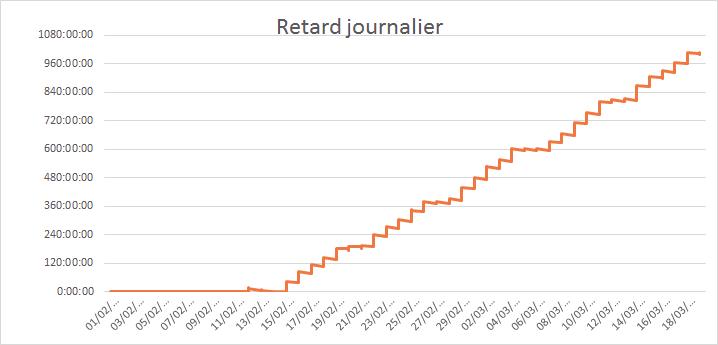
\includegraphics[scale=0.6]{retard_jour.png}
 \caption{\label{retard_jour_8} Retard avec 8 portes} 
\end{figure}
 
 \subsection{Aéroport à 12 portes d'embarquement}
La répartition des retards pour un aéroport à 12 portes,en pourcentage d'avions dans des intervalles de retards est donnée en figure~\ref{retard_camenbert_12}.
  \graphicspath{{donnees/graph_90jours/12portes/}}
\begin{figure}[H]
\centering 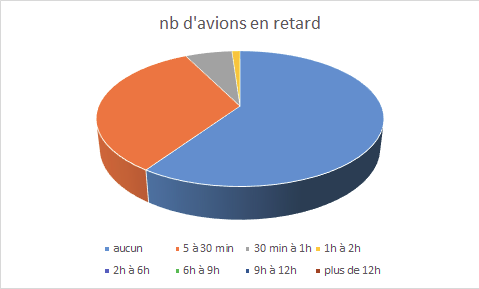
\includegraphics[scale=0.6]{retard_avions.png}
 \caption{\label{retard_camenbert_12} Répartition des retards, avec 12 portes} 
\end{figure}
 
 Une autre donnée intéressante est la répartition des retards par jour, donnée par la figure~\ref{retard_jour_12}
\begin{figure}[H]
\centering 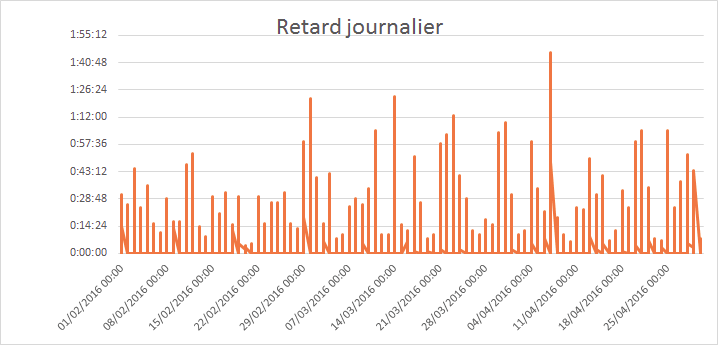
\includegraphics[scale=0.6]{retard_jour.png}
 \caption{\label{retard_jour_12} Retard avec 12 portes} 
\end{figure}
 
\section{Répartition journalière des arrivées}
Quelque soit le nombre de portes, les nombres moyens d'atterrissage par heure --respectivement en jour de semaine et en week-end-- restent les mêmes, tels que donnés dans les figures~\ref{arrivee_semaine} et~\ref{arrivee_we}.

\begin{figure}[H]
\centering 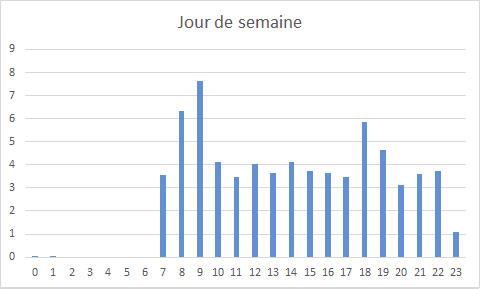
\includegraphics[scale=0.6]{arrivee_semaine.png}
 \caption{\label{arrivee_semaine} Quantité d'atterrissage par horaires en semaine} 
\end{figure}
 
\begin{figure}[H]
\centering 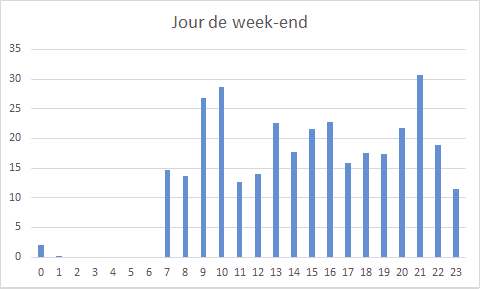
\includegraphics[scale=0.6]{arrivee_we.png}
 \caption{\label{arrivee_we} Quantité d'atterrissage par horaires le week-end} 
\end{figure}
